\documentclass[tikz, border=4pt]{standalone}

% --- packages (mirror these in adc-triangle.meta.json "requires") ---
\usepackage{tikz}
\usetikzlibrary{shapes.geometric}

% --- palette (canonical source: reference/color-palettes/color-palettes.md; light variant) ---
\definecolor{otgray}{HTML}{5A5A5A}
% --- ESL domain-semantic tokens (contract §2, ADR-0005 D7) ---
\colorlet{digitaldomain}{gray}

\begin{document}
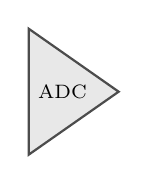
\begin{tikzpicture}
  % contract §1a `adc`: "analog->digital converter, drawn as a small apex-right
  % triangle" -- an isosceles triangle at shape border rotate=0 already points
  % its apex right (the default orientation), so no rotation is needed. Filled
  % with digitaldomain: the ADC's OUTPUT is the digital word this feeds.
  \node[isosceles triangle, isosceles triangle apex angle=70,
        draw=otgray!85!black, thick, fill=digitaldomain!18,
        minimum height=1.05cm, minimum width=1.05cm,
        font=\scriptsize] (adc) {ADC};
\end{tikzpicture}
\end{document}
